\documentclass[tikz,border=10pt]{standalone}
\begin{document}
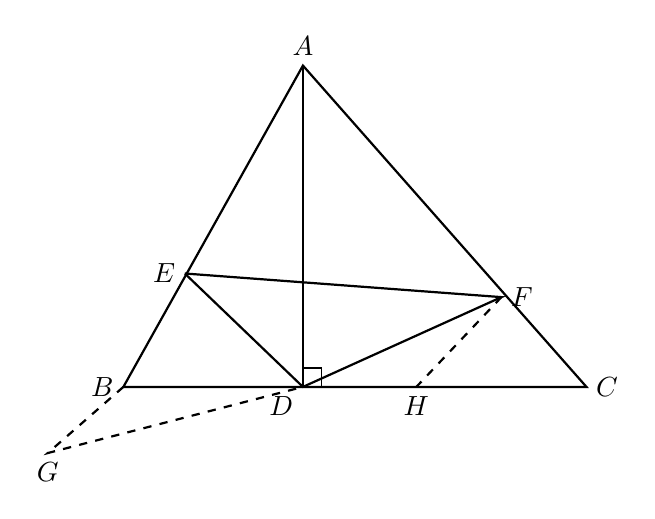
\begin{tikzpicture}[scale=1.2]
\coordinate (A) at (2.4,4.2);
\coordinate (B) at (0.5,0.8);
\coordinate (C) at (5.4,0.8);
\coordinate (D) at (2.4,0.8);
\coordinate (E) at (1.15,2.0);
\coordinate (F) at (4.5,1.75);
\coordinate (G) at (-0.3,0.1);
\coordinate (H) at (3.6,0.8);

\draw[thick] (A) -- (B) -- (C) -- cycle;
\draw[thick] (A) -- (D);
\draw[thick] (E) -- (D) -- (F) -- (E);
\draw[thick,dashed] (B) -- (G) -- (D);
\draw[thick,dashed] (F) -- (H);

\draw (2.4,1.0) -- (2.6,1.0) -- (2.6,0.8) -- (2.4,0.8) -- cycle;

\node[above] at (A) {$A$};
\node[left] at (B) {$B$};
\node[right] at (C) {$C$};
\node[below left] at (D) {$D$};
\node[left] at (E) {$E$};
\node[right] at (F) {$F$};
\node[below] at (G) {$G$};
\node[below] at (H) {$H$};
\end{tikzpicture}
\end{document}
